\hypertarget{test__match2_8cpp}{}\subsection{test\+\_\+match2.\+cpp File Reference}
\label{test__match2_8cpp}\index{test\+\_\+match2.\+cpp@{test\+\_\+match2.\+cpp}}


Contains an example to take subject string, pattern and modifier from user input and perform regex match using J\+P\+C\+R\+E2.  


{\ttfamily \#include $<$iostream$>$}\\*
{\ttfamily \#include \char`\"{}jpcre2.\+hpp\char`\"{}}\\*
Include dependency graph for test\+\_\+match2.\+cpp\+:\nopagebreak
\begin{figure}[H]
\begin{center}
\leavevmode
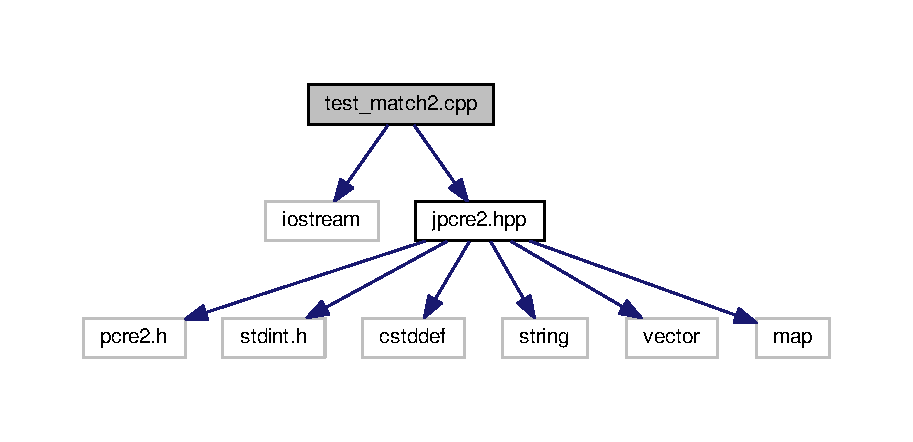
\includegraphics[width=350pt]{test__match2_8cpp__incl}
\end{center}
\end{figure}


\subsubsection{Detailed Description}
Contains an example to take subject string, pattern and modifier from user input and perform regex match using J\+P\+C\+R\+E2. 


\begin{DoxyCodeInclude}
\textcolor{comment}{/**@file test\_match2.cpp}
\textcolor{comment}{ * Contains an example to take subject string, pattern and modifier}
\textcolor{comment}{ * from user input and perform regex match using JPCRE2.}
\textcolor{comment}{ * @include test\_match2.cpp}
\textcolor{comment}{ * @author [Md Jahidul Hamid](https://github.com/neurobin)}
\textcolor{comment}{ * */}

\textcolor{preprocessor}{#include <iostream>}
\textcolor{preprocessor}{#include "\hyperlink{jpcre2_8hpp}{jpcre2.hpp}"}


\textcolor{preprocessor}{#define getLine(a) std::getline(std::cin,a,'\(\backslash\)n')}


\textcolor{keywordtype}{int} main()\{

    \hyperlink{namespacejpcre2_ac1cf752c8fbb0be78020be3b80e77ce3}{jpcre2::VecNum} vec\_num0;   \textcolor{comment}{///Vector to store numbered substring Map.}
\textcolor{comment}{}    \hyperlink{namespacejpcre2_a2b121ae776ea5b2913839f418a7d856b}{jpcre2::VecNas} vec\_nas0;   \textcolor{comment}{///Vector to store named substring Map.}
\textcolor{comment}{}    \hyperlink{namespacejpcre2_a88a7aaf84cad627d34c8152e726168eb}{jpcre2::VecNtN} vec\_nn0;    \textcolor{comment}{///Vector to store Named substring to Number Map.}
\textcolor{comment}{}    
   
    std::string pat,mod,subject;
    \textcolor{comment}{}
\textcolor{comment}{    ///create an object}
\textcolor{comment}{}    \hyperlink{classjpcre2_1_1Regex}{jpcre2::Regex} re;     \textcolor{comment}{/// This should not throw any exception}
\textcolor{comment}{}
    std::cout<<\textcolor{stringliteral}{"Enter pattern: "};
    getLine(pat);
    cp:
    std::cout<<\textcolor{stringliteral}{"Enter compile modifiers (eijmnsuxADJSU): "};
    getLine(mod);
    \textcolor{comment}{}
\textcolor{comment}{    ///Compile pattern}
\textcolor{comment}{}    \textcolor{keywordflow}{try}\{re.\hyperlink{classjpcre2_1_1Regex_aad1d5ef1e87f762f68a587eec4022e69}{compile}(pat,mod);\}
    \textcolor{keywordflow}{catch}(\textcolor{keywordtype}{int} e)\{std::cerr<<re.\hyperlink{classjpcre2_1_1Regex_a92b75c438ccff871205b2175a6141fd5}{getErrorMessage}(e)<<std::endl;\textcolor{keywordflow}{goto} cp;\}
           
    \textcolor{comment}{/******************************************************************************************************
      *********}
\textcolor{comment}{     * Use try catch block to catch any exception and avoid unexpected termination of the program in case
       of error}
\textcolor{comment}{     * All jpcre2 exceptions are of type int (integer)}
\textcolor{comment}{     * ****************************************************************************************************
      *********/}
    
\textcolor{comment}{}
\textcolor{comment}{    ///subject string}
\textcolor{comment}{}    std::cout<<\textcolor{stringliteral}{"\(\backslash\)nEnter subject string (enter quit to quit): "}<<std::endl;
    getLine(subject);
    std::string ac\_mod;

    \textcolor{keywordtype}{size\_t} matched = 0;\textcolor{comment}{}
\textcolor{comment}{    /// Continue loop as long as error occurs}
\textcolor{comment}{}    \textcolor{keywordflow}{while}(\textcolor{keyword}{true})\{
        std::cout<<\textcolor{stringliteral}{"\(\backslash\)nEnter action (matching) modifier (Ag): "}<<std::endl;
        getLine(ac\_mod);
        \textcolor{keywordflow}{if}(subject==\textcolor{stringliteral}{"quit"})\textcolor{keywordflow}{return} 0;
        \textcolor{keywordflow}{try}\{matched=re.\hyperlink{classjpcre2_1_1Regex_a519b0915bf1163c6ce6a4d674b30cfcd}{initMatch}()                                \textcolor{comment}{//Invoke the initMatch()
       function}
                      .\hyperlink{classjpcre2_1_1RegexMatch_a9df7e92f96b61553f62720cb8f5f23e5}{setModifier}(ac\_mod)                        \textcolor{comment}{//Set various options}
                      .\hyperlink{classjpcre2_1_1RegexMatch_a2c7efe1ec2e13827f670db4ecedcd0a0}{setNumberedSubstringVector}(&vec\_num0)      \textcolor{comment}{//...}
                      .\hyperlink{classjpcre2_1_1RegexMatch_ae495431f57cae54363331237ab21b56c}{setNamedSubstringVector}(&vec\_nas0)         \textcolor{comment}{//...}
                      .\hyperlink{classjpcre2_1_1RegexMatch_a04926e61d8b5f1d8bdf344efecd567d8}{setNameToNumberMapVector}(&vec\_nn0)         \textcolor{comment}{//...}
                      .\hyperlink{classjpcre2_1_1RegexMatch_a0a4cf8554a7e00f3cf2db34f60a43f60}{addJpcre2Option}(\hyperlink{namespacejpcre2_a85c143271501e383843f45b9999c2f00a9124b768bcae4d51430aa7f26126f387}{jpcre2::VALIDATE\_MODIFIER}) \textcolor{comment}{
      //...}
                      .\hyperlink{classjpcre2_1_1RegexMatch_aac4857cd8f5eae15b29b9afbe9023522}{addPcre2Option}(0)                          \textcolor{comment}{//...}
                      .\hyperlink{classjpcre2_1_1RegexMatch_a5868aef3a146594ea1ebef34d122bb33}{match}();                                   \textcolor{comment}{//Finally do the match}
        \}
        \textcolor{keywordflow}{catch}(\textcolor{keywordtype}{int} e)\{std::cerr<<re.\hyperlink{classjpcre2_1_1Regex_a92b75c438ccff871205b2175a6141fd5}{getErrorMessage}(e);
            \textcolor{keywordflow}{if}(e==\hyperlink{namespacejpcre2_1_1ERROR_a4b2998984439438fa9da8d7043909bc2a4115340549b623f4e2da285bf0aa9bff}{jpcre2::ERROR::INVALID\_MODIFIER}) \textcolor{keywordflow}{continue};
        \}
        \textcolor{keywordflow}{break};
    \}\textcolor{comment}{}
\textcolor{comment}{    ///Now let's access the matched data}
\textcolor{comment}{}\textcolor{comment}{}
\textcolor{comment}{    ///Each of these vectors contains maps.}
\textcolor{comment}{    ///Each element in the vector specifies a particular match}
\textcolor{comment}{    ///First match is the vector element 0, second is at index 1 and so forth}
\textcolor{comment}{    ///A map for a vector element, i.e for a match contains all of its substrings/capture groups}
\textcolor{comment}{    ///The first element of the map is capture group 0 i.e total match}
\textcolor{comment}{}    std::cout<<\textcolor{stringliteral}{"\(\backslash\)nTotal number of matches: "}<<matched<<std::endl;
    \textcolor{keywordflow}{if}(matched)\{
        \textcolor{keywordflow}{for}(\textcolor{keywordtype}{size\_t} i=0;i<vec\_num0.size();++i)\{
            
            
            std::cout<< \textcolor{stringliteral}{"\(\backslash\)n################## Match no: "}<<i+1<<\textcolor{stringliteral}{" ####################\(\backslash\)n"};
            
            
            \textcolor{comment}{}
\textcolor{comment}{            ///This vector contains maps with number as the key and the corresponding substring as the
       value}
\textcolor{comment}{}            std::cout<<\textcolor{stringliteral}{"\(\backslash\)n-------------------------------------------------------------------------"};
            std::cout<< \textcolor{stringliteral}{"\(\backslash\)n--- Numbered Substrings (number: substring) for match "}<<i+1<<\textcolor{stringliteral}{" ---\(\backslash\)n"};
            \textcolor{keywordflow}{for}(jpcre2::MapNum::iterator ent=vec\_num0[i].begin();ent!=vec\_num0[i].end();++ent)\{
                std::cout<<\textcolor{stringliteral}{"\(\backslash\)n\(\backslash\)t"}<<ent->first<<\textcolor{stringliteral}{": "}<<ent->second<<\textcolor{stringliteral}{"\(\backslash\)n"};
            \}
            
            
            \textcolor{comment}{}
\textcolor{comment}{            ///This vector contains maps with name as the key and the corresponding substring as the value}
\textcolor{comment}{}            std::cout<<\textcolor{stringliteral}{"\(\backslash\)n-------------------------------------------------------------------------"};
            std::cout<< \textcolor{stringliteral}{"\(\backslash\)n--- Named Substrings (name: substring) for match "}<<i+1<<\textcolor{stringliteral}{" ---\(\backslash\)n"};
            \textcolor{keywordflow}{for}(jpcre2::MapNas::iterator ent=vec\_nas0[i].begin();ent!=vec\_nas0[i].end();++ent)\{
                std::cout<<\textcolor{stringliteral}{"\(\backslash\)n\(\backslash\)t"}<<ent->first<<\textcolor{stringliteral}{": "}<<ent->second<<\textcolor{stringliteral}{"\(\backslash\)n"};
            \}
            
            
            \textcolor{comment}{}
\textcolor{comment}{            ///This vector contains maps with name as the key and number as the value}
\textcolor{comment}{            ///i.e the number (of substring) can be accessed with the name for named substring.}
\textcolor{comment}{}            std::cout<<\textcolor{stringliteral}{"\(\backslash\)n-------------------------------------------------------------------------"};
            std::cout<< \textcolor{stringliteral}{"\(\backslash\)n--- Name to number mapping (name: number/position) for match "}<<i+1<<\textcolor{stringliteral}{" ---\(\backslash\)n"};
            \textcolor{keywordflow}{for}(jpcre2::MapNtN::iterator ent=vec\_nn0[i].begin();ent!=vec\_nn0[i].end();++ent)\{
                std::cout<<\textcolor{stringliteral}{"\(\backslash\)n\(\backslash\)t"}<<ent->first<<\textcolor{stringliteral}{": "}<<ent->second<<\textcolor{stringliteral}{"\(\backslash\)n"};
            \}
        \}
    \}
    \textcolor{keywordflow}{else} std::cout<<\textcolor{stringliteral}{"\(\backslash\)nNo match found\(\backslash\)n"};
    \textcolor{comment}{//main();}
    \textcolor{keywordflow}{return} 0;
\}
\end{DoxyCodeInclude}
 \begin{DoxyAuthor}{Author}
\href{https://github.com/neurobin}{\tt Md Jahidul Hamid} 
\end{DoxyAuthor}
